\documentclass[11pt,a4paper]{article}
\usepackage[utf8]{inputenc}
\usepackage[T1]{fontenc}
\usepackage[margin=2.2cm]{geometry}
\usepackage{booktabs}
\usepackage{array}
\usepackage{tabularx}
\usepackage{longtable}
\usepackage{multirow}
\providecommand{\num}[1]{#1}
\usepackage{hyperref}
\hypersetup{colorlinks=true,linkcolor=black,urlcolor=blue}
\usepackage{xcolor}
\usepackage{graphicx}
\usepackage{amsmath}
\usepackage{enumitem}
\setlist{nosep,leftmargin=*}

\title{Vision--Language Models on the VLM-eval-rcp\\driving-video benchmark:\\
a ten-model audit of failure modes\\and the agentic gap}
\author{Matthieu Scharffe}
\date{May 2026}

\newcommand{\pct}[1]{#1\,\%}
\newcommand{\code}[1]{\texttt{#1}}

\begin{document}
\maketitle

\begin{abstract}
We extend two prior single-model audits (GPT-5.4-mini, Gemini~3~Flash) into
a uniform cross-model failure analysis of \textbf{ten} vision--language
configurations on the VLM-eval-rcp driving-video benchmark
(\num{7371} (video, question) pairs, six categories, five JPEG frames at
1\,fps per clip). Eight new systems are added: six open-source baselines
(Cosmos-Reason, InternVL3.5-8B/30B, LLaVA-OneVision, Qwen3-VL,
Qwen2.5-Omni) and two agentic Qwen3-VL configurations (with and without
hint scaffolding). Overall accuracy ranges from \pct{21.9} (Qwen3-VL) to
\pct{64.0} (Gemini~3~Flash). Open-source baselines cluster between
\pct{22} and \pct{31}; the bare agent (v4o) is at \pct{60.1} and the
hinted agent (v4p) at \pct{50.9}. Per-category analysis isolates six
failure modes that recur across~$\geq$~5 models: a near-deterministic
``Real'' prior on generation detection, Likert mode-collapse on the
midpoint or upper bin, a constant-``Yes'' classifier on
violation-heavy traffic-rules questions, continuous-motion attribution
that denies generative artefacts, ego-relative reference-frame
inversion on overtake-side, and absence-of-evidence reasoning that
infers compliance from the lack of a visible incident. The agent route
shifts the regime by replacing language-prior reasoning with a
frequency-domain anisotropy threshold (FFT) and an optical-flow priority
rule (SOP-C) that promote tool-measured cues above heuristic checklists;
hint scaffolding helps only on traffic-laws (where it furnishes the
violation vocabulary the bare agent lacks) and otherwise re-imports the
absence-of-evidence trap. Gemini~3~Flash matches the agent without
tools by combining a learned generative-artefact taxonomy
(``morphing'', ``mushy textures'', ``physically implausible lens
flare'') with frame-pair object-permanence reasoning and strong OCR on
near-English signage --- a profile no open baseline currently produces.
\end{abstract}

\section{Setup}
\label{sec:setup}

\paragraph{Benchmark.} The harness joins each model's per-record
output against the two ground-truth question files
(\code{questions\_cosmos-drive-dreams} and the
\code{cosmos-predict1} sibling), parses an answer from the
benchmark's mandated \emph{``Feedback::: / Evaluation: /
Answer:~\dots''} response shape, and computes accuracy plus per-source,
per-category, per-question and per-cell confusion tables. For the
six open-source baselines whose \code{vlm\_answer} column was stored
as the unparsed full output we re-extract the final ``Answer:''
token via a last-occurrence regex with question-aware Yes/No, 1--3,
Real/Generated and Left/Right fallbacks. The agentic v4o/v4p systems
already emit a structured \code{final\_answer} field. The pipeline
script writes one enriched parquet per model plus a single
accuracy-summary JSON.

\paragraph{Sources.} Videos come from two splits.
\emph{cosmos-drive-dreams} (\num{6385} answered questions per system,
folders \code{negative/}, \code{aggressive\_takeover/},
\code{crossing\_red\_lights/}, \code{crossing\_stop/}) contains
photoreal world-model output. \emph{cosmos-predict1} (\num{986}, folder
\code{artifacts/}) contains clips with visible diffusion artefacts and
supplies the entire Artefacts-understanding category, all 727 of its
items. Reality understanding draws from both sources (2186
drive-dreams + 986 predict1). Every Reality-binary item has
GT~$=$~\emph{Generated}; the realism Likert is in $\{1,2\}$; the safety
Likert is in $\{1,2,3\}$; the artefacts and traffic-rules questions are
heavily skewed (\pct{88} GT~$=$~Yes on artefacts, \pct{99} GT~$=$~No on
``following traffic rules''). These priors are exploitable, and several
models do exploit them, which we flag throughout.

\paragraph{Models.} Ten configurations, eight evaluated in this work and
two contributed by prior single-model audits we synthesise alongside.
We refer to them by short identifier (Tables~\ref{tab:overall},
\ref{tab:cat}).

\section{Headline accuracy}
\label{sec:headline}

Table~\ref{tab:overall} sorts the ten configurations by overall
accuracy. Three regimes coexist: (i) open-source baselines clustered in
the \pct{22}--\pct{31} band, (ii) two closed-source single-pass models
(GPT-5.4-mini at \pct{39.1}, Gemini~3~Flash at \pct{64.0}), (iii) the
agentic Qwen3-VL pipeline (\pct{60.1} bare, \pct{50.9} hinted) which
matches Gemini on the categories where its tools fire but trails it on
near-saturated single-frame questions. Table~\ref{tab:cat} breaks the
score down by category and exposes that no model dominates uniformly:
even Gemini sits below the agentic systems on ``Has the ego car
stopped?'' (Spatial-temporal) and below GPT-5.4-mini on Visual
understanding.

\begin{figure}[h]
\centering
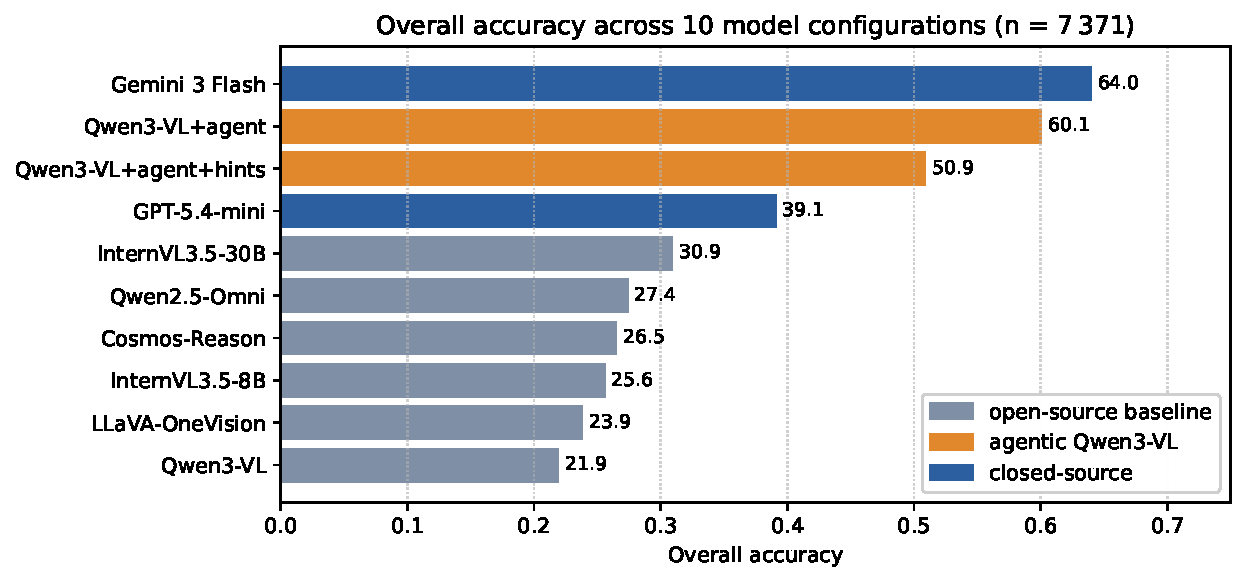
\includegraphics[width=0.95\linewidth]{fig_overall_accuracy.pdf}
\caption{Overall accuracy across the ten configurations on the
\num{7371}-pair evaluation set. Open-source baselines (grey) cluster in
the \pct{22}--\pct{31} band; the agentic Qwen3-VL pipeline (orange)
sits at \pct{60.1} bare and \pct{50.9} hinted; closed-source models
(blue) sit at \pct{39.1} (GPT-5.4-mini) and \pct{64.0} (Gemini~3
Flash).}
\label{fig:overall}
\end{figure}

\begin{figure}[h]
\centering
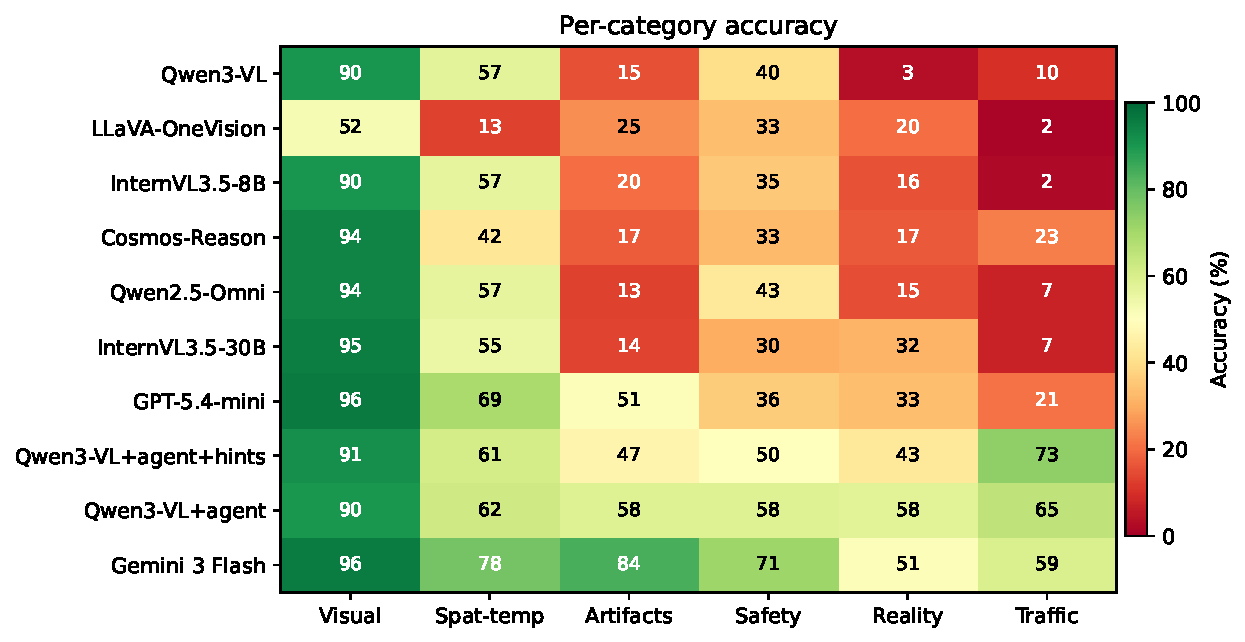
\includegraphics[width=0.98\linewidth]{fig_per_category.pdf}
\caption{Per-category accuracy. Visual understanding is near-saturated
for nine of ten configurations (LLaVA-OneVision is the outlier);
Reality / Artefacts / Traffic-laws are where the open-source baselines
collapse and where the agent route or Gemini's pre-trained
artefact taxonomy provides the lift.}
\label{fig:cat}
\end{figure}

\begin{table}[h]
\centering
\begin{tabular}{lrr}
\toprule
Model & $n$ & Accuracy \\
\midrule
Qwen3-VL                         & 7371 & \pct{21.92} \\
LLaVA-OneVision                  & 7371 & \pct{23.85} \\
InternVL3.5-8B                   & 7371 & \pct{25.61} \\
Cosmos-Reason                    & 7371 & \pct{26.54} \\
Qwen2.5-Omni                     & 7371 & \pct{27.43} \\
InternVL3.5-30B                  & 7371 & \pct{30.93} \\
GPT-5.4-mini\,$^\dagger$         & 7282 & \pct{39.12} \\
Qwen3-VL\,+\,agent\,+\,hints (v4p) & 7371 & \pct{50.93} \\
Qwen3-VL\,+\,agent (v4o)         & 7371 & \pct{60.07} \\
Gemini 3 Flash\,$^\dagger$       & 7282 & \pct{64.00} \\
\bottomrule
\end{tabular}
\caption{Overall accuracy on the 7\,371-pair evaluation set. Daggered
rows are reproduced from prior single-model audits (joined-record
counts differ because of OpenAI batch-API failures and a small number
of unparseable Gemini calls).}
\label{tab:overall}
\end{table}

\begin{table}[h]
\centering
\small
\begin{tabular}{lrrrrrr}
\toprule
Model & Visual & Spatial-temp & Artifacts & Safety & Reality & Traffic \\
& {(304)} & {(339)} & {(727)} & {(2164)} & {(3172)} & {(665)} \\
\midrule
Qwen3-VL                & 90.5 & 57.2 & 15.3 & 39.9 &  3.5 &  9.8 \\
LLaVA-OneVision         & 52.3 & 13.0 & 25.2 & 33.4 & 20.1 &  1.5 \\
InternVL3.5-8B          & 90.5 & 56.6 & 20.1 & 35.4 & 15.6 &  2.0 \\
Cosmos-Reason           & 94.1 & 42.5 & 17.5 & 32.6 & 17.0 & 23.0 \\
Qwen2.5-Omni            & 94.1 & 56.6 & 13.1 & 42.7 & 15.1 &  7.1 \\
InternVL3.5-30B         & 95.1 & 54.9 & 13.6 & 30.3 & 31.6 &  7.2 \\
GPT-5.4-mini            & 95.7 & 69.0 & 50.9 & 36.3 & 33.5 & 20.8 \\
v4p (agent + hints)     & 91.4 & 60.8 & 46.8 & 50.2 & 42.8 & \textbf{73.1} \\
v4o (agent)             & 90.1 & 61.9 & \textbf{58.5} & \textbf{58.3} & \textbf{57.5} & 65.0 \\
Gemini 3 Flash          & \textbf{95.7} & \textbf{77.6} & \textbf{83.9} & \textbf{71.0} & 51.1 & 59.4 \\
\bottomrule
\end{tabular}
\caption{Per-category accuracy (\%) for the ten configurations. Item
counts in the header. Column-bests in bold; ties broken in favour of
the model that does not use tools. Note that on Visual and
Spatial-temporal, every model except LLaVA is near-saturated, so the
column-best is essentially noise.}
\label{tab:cat}
\end{table}

\section{Cross-model failure modes}
\label{sec:modes}

Six failure modes recur across $\geq 5$ of the ten configurations and
account for the bulk of the absolute error count. We list them in
decreasing order of total error mass.

\paragraph{(M1) ``Real'' prior on generation detection.} Across the six
open-source baselines, the binary \emph{Is it a real video or
generated?} produces between \num{1291} and \num{1597} false negatives
out of \num{1597} items, i.e. a false-negative rate from \pct{80.8}
(Cosmos-Reason) to \pct{100.0} (LLaVA-OneVision; \pct{99.3} for
Qwen3-VL). The reasoning is uniformly absence-of-artefact reasoning:
\emph{``no obvious signs of digital artifacts or inconsistencies that
would suggest it is generated by AI''} (Qwen3-VL,
\code{negative/agg\_tk\_030\_Foggy.mp4}); \emph{``Generated videos
often have subtle but noticeable artifacts\,\dots\,this video does not
display such signs''} (InternVL3.5-30B,
\code{cross\_red\_036\_Original.mp4}). The ``mental checklist''
(warping, flicker, duplication) is tuned to GAN-era tells while the
clips are diffusion-based world-model output specifically engineered
to remove them. GPT-5.4-mini and the bare Qwen3-VL show the same
profile (FN rates \pct{88.9} and \pct{99.3}); Gemini cuts it to
\pct{44.6}; the agent route cuts it to \pct{25.4} (v4o) by replacing
the language prior with a frequency-domain anisotropy test
(\S\ref{sec:agent}).

\paragraph{(M2) Likert mode-collapse.} The 1--3 Likert questions
(realism and safety) collapse to one or two of three labels in nine of
ten configurations. Cosmos-Reason, InternVL3.5-30B, InternVL3.5-8B and
LLaVA-OneVision each emit ``2'' on $\geq$\,\pct{81} of all safety-Likert
items (Cosmos: 970/1082; InternVL-30B: 1011/1082); since the safety GT
is dominated by the extremes (485 GT~$=$~1, 597 GT~$=$~3), a constant-2
strategy floors them at \pct{8}--\pct{13}. Qwen3-VL and Qwen2.5-Omni
collapse onto \{2,3\} but never emit ``1''. GPT-5.4-mini emits ``1'' zero
times on the safety Likert. Gemini emits ``2'' essentially never (31
GT~$=$~2 cases out of 1553 makes the middle class nearly untestable, but
its predictions concentrate on \{1,3\}, with 245 of 334 score-task errors
being the maximally-wrong $\text{GT}=1\to\text{VLM}=3$). The bare agent
(v4o) is the only system that emits ``1'' at a meaningful rate (121
times) and the only one whose safety-Likert accuracy
(\pct{50.9}) exceeds the binary floor; the hinted agent regresses to 16
ones (\S\ref{sec:hints}).

\paragraph{(M3) Constant-``Yes'' on traffic-rules.} On \emph{Is the ego
car following the traffic rules?} (n~$=$~512, GT~$=$~No in 510), the
six baselines answer Yes between \pct{82} and \pct{100} of the time on
GT~$=$~No clips: LLaVA-OneVision 655/655 (recall on No is exactly~0),
InternVL3.5-8B 652/665, Qwen2.5-Omni 618/655, InternVL3.5-30B 617/655,
Qwen3-VL 600/655, Cosmos-Reason 503/645. GPT-5.4-mini and Gemini show
the same direction at lower magnitude (\pct{82.2} and \pct{52.4}
FP-on-No respectively). The mechanism is a templated checklist
(``safe distance / within lane / following traffic flow'') reached by
absence-of-evidence reasoning: \emph{``no visible signs of
reckless driving''} (Qwen2.5-Omni, \code{agg\_tk\_017\_Night.mp4}). The
violation vocabulary is restricted to overt, single-frame events
(speeding, lane change, red-light, stop sign), so trajectory-encoded
violations (cut-offs, tailgating, shoulder driving, rolling stops) never
trigger a~No.

\paragraph{(M4) Continuous-motion attribution on artefacts.} On
\emph{Does any object appear or disappear without continuous motion?},
the phrase \emph{``continuous motion''} appears in \pct{33}--\pct{41} of
every base-model failure file (Qwen2.5-Omni 257/632, LLaVA 231/544,
Cosmos-Reason 239/600). Steady forward camera flow is read as a license
to deny any inter-frame discontinuity: \emph{``all objects \dots\ are
visible throughout the sequence without sudden appearances or
disappearances''} (Qwen3-VL, \code{cross\_stop\_003\_Night.mp4}). The
related \emph{stable-silhouette $\Rightarrow$ no artefact} heuristic
(``maintain their shape'' in $\sim$~\pct{40}--\pct{45} of Qwen-family
failures) collapses identity-preservation onto rigidity, missing
texture flicker, identity drift and material inconsistency. Together
these two heuristics produce constant-No classifiers in five of six
baselines (Qwen3-VL emits exactly zero ``Yes'' across 616 artefact
failures; InternVL3.5-30B emits 1).

\paragraph{(M5) Reference-frame inversion on overtake-side.} On
\emph{On which side is the ego car overtaking?} every model that
commits to a side flips it. Across the eight in-house systems plus
GPT-5.4-mini and Gemini, the modal failure is a coherent ego-relative
description in the chain-of-thought followed by an inverted label:
\emph{``moving from the right lane to the left lane to overtake them''}
$\to$~Left, GT~Right (InternVL3.5-30B,
\code{agg\_tk\_015\_Night.mp4}); \emph{``passes a black truck on the
right between frames~1 and~2 \dots\ overtaking on the left''} (Gemini,
\code{agg\_tk\_017\_Rainy.mp4}). The benchmark labels the lane the
ego \emph{enters} (or equivalently the side of the overtaken vehicle);
the models label the side of the ego relative to the overtaken vehicle.
The two conventions are opposites, so every coherent perception flips.
The agent route does not help (v4o \pct{12.0}; v4p \pct{6.8}) because
the failure is downstream of perception --- the labelling step, not the
optical-flow tool. A single-sentence prompt clarification would
recover most of this category.

\paragraph{(M6) Absence-of-evidence as compliance / safety.} The
unifying error pattern across Reality, Safety, Traffic-laws and
Artefacts is the inference \emph{absent visible violation
$\Rightarrow$~compliant / safe / authentic / artefact-free}. Examples
appear above for each category; the structural pattern is that all
ten configurations enumerate what is \emph{not} present and conclude
the non-violation answer. The 5-frame/1-fps temporal budget makes this
worse: every category whose answer requires inter-frame reasoning
(stop-line traversal, takeover dynamics, brief artefact pop) interpolates
a compliant state-change between sampled frames rather than flagging
the ambiguity. This single mode is the largest absolute error source in
every system except the bare agent.

\section{Per-category briefs}
\label{sec:briefs}

The per-category audits behind these summaries are in
\code{baseline\_analysis/reports/*.md}; here we keep only the
cross-model contrasts that paper readers need.

\paragraph{Reality understanding (3172 items; 2186 drive-dreams + 986
predict1).} Five of six baselines sit between \pct{15} and \pct{32};
Qwen3-VL is at \pct{3.5}. InternVL3.5-30B is the strongest non-agent
at \pct{31.6}, but the lift is entirely Likert mode-collapse on ``2'':
\pct{56.4} on the realism Likert versus \pct{7.3} on the binary.
Cosmos-Reason has the highest binary accuracy among baselines
(\pct{19.0}) thanks to a working --- if low-recall ---
generative-artefact taxonomy that occasionally catches \emph{``the
unnatural behavior\,\dots\ could indicate something artificial''}
(Cosmos-Reason, \code{7f3bbe35\dots\_Morning.mp4}). Per-source
asymmetry is universal: every system scores worse on
\emph{cosmos-predict1} than on \emph{cosmos-drive-dreams}, by
$5$--$30$ points (LLaVA: \pct{29.2} vs \pct{0.1}; InternVL3.5-30B:
\pct{42.5} vs \pct{7.6}; v4o agent: \pct{62.1} vs \pct{47.5}).
Counter-intuitively the lower-fidelity source is harder to call
``Generated'': the binary GT is the same on both, but cosmos-predict1
clips lack the world-model's frequency-domain signature that triggers
the agent's FFT cue, and their visible morphs are exactly what every
baseline's stable-silhouette excuse dismisses. The agent's binary
accuracy is \pct{74.6} and is driven almost entirely by an FFT
anisotropy threshold (\S\ref{sec:agent}); Gemini's \pct{55.4} is driven
by OCR on near-English signage (\emph{``the morphing of the `STOPP'
text on the road''}, \emph{``the `PARKING' sign \dots\ morphing into
`PANNI' ''}, \emph{``PALCONERI''}, \emph{``STNULL - STNAID''}).

\paragraph{Safety understanding (2164 items).} Six baselines cluster
between \pct{30.3} and \pct{42.7}; the binary task is essentially a
``Yes'' classifier for all of them (\pct{50.6}--\pct{57.9}, only
marginally above the \pct{52.6} Yes-prior). The Likert is the divider:
v4o jumps to \pct{50.9}, every baseline stays at \pct{8}--\pct{29}. The
mechanism behind v4o's lift is concentrated:
\code{crossing\_red\_lights/} Likert goes from \pct{0.7} to \pct{58.6}
and \code{negative/} from \pct{47.6} to \pct{78}, while
\code{crossing\_stop/} (\pct{8.4}~$\to$~\pct{8.4}) and
\code{aggressive\_takeover/} (\pct{0.0}~$\to$~\pct{0.6}) are unchanged.
Gemini's \pct{71.0} matches the agent on red-lights and stops via
static-cue reading and beats it on \code{negative/} clips, but
collapses on \code{aggressive\_takeover/} to \pct{19.3} for the same
trajectory-blindness reason as the baselines.

\paragraph{Traffic laws (665 items).} Open baselines collapse to
\pct{1.5}--\pct{23.0}. Cosmos-Reason is the strongest (\pct{23.0})
because it is the only baseline that emits ``No'' more than 100 times
($n=$~145 vs.~3--40 for peers) and has a working stop-sign rule chain.
The agent route lifts Qwen3-VL by 54 points
(\pct{9.8}~$\to$~\pct{65.0}) entirely on red-lights and stops; the
hinted agent (v4p) climbs further to \pct{73.1} ---
\textbf{the only category in the benchmark where v4p beats v4o} ---
because the violation-targeted hint payload furnishes the missing
``cut-off / unsafe overtake'' vocabulary (\S\ref{sec:hints}).
\code{aggressive\_takeover/} accuracy on follow-rules: \pct{5.6}
(baseline) $\to$~\pct{5.6} (v4o) $\to$~\pct{85.6} (v4p), at the cost
of $-$\pct{22.5} on red-lights and $-$\pct{20.9} on stops.

\paragraph{Artifacts understanding (727 items, GT~$=$~Yes in 88\%).}
Five of six baselines sit in the constant-No band (\pct{13}--\pct{20});
LLaVA's \pct{25.2} is mechanically explained by a \pct{17} Yes-rate
(precision-on-Yes \pct{90.2} matches the GT prior), not detection.
InternVL3.5-30B underperforms its 8B sibling (\pct{13.6} vs
\pct{20.1}) because the larger model's RLHF alignment sharpens the
``don't fabricate'' prior --- the wrong default on a Yes-skewed
benchmark. The agent reaches \pct{58.5} via FFT anisotropy and SAM-mask
rigidity-violation vocabulary (\emph{``texture swimming''},
\emph{``components morphing''}, \emph{``wheels warp and merge into the
body''}). Gemini reaches \pct{83.9} \emph{without tools} via per-frame
OCR on garbled signage, frame-pair object-permanence reasoning
(``between frames 4 and 5\,\dots'') and a learned named taxonomy
(\emph{``mushy textures''}, \emph{``physically implausible lens
flare''}). It is the single category where Gemini beats the agent by
a wide margin (\S\ref{sec:gemini}).

\paragraph{Spatial-temporal (339 items).} Two questions: ``Has the ego
car stopped?'' (n~$=$~201; six of eight near-saturated, LLaVA at
\pct{8.5}, Cosmos-Reason at \pct{52.7}) and ``On which side is the ego
car overtaking?'' (n~$=$~133, GT~$=$~Right in 127). The overtake-side
question is mode~M5 in pure form. LLaVA's stop-question collapse
(\pct{8.5}) is a constant-Yes anchored to the visible STOP sign rather
than to inter-frame motion: \emph{``the ego car has stopped \dots\ as
indicated by the `STOP' sign visible in the video''}
(\code{cross\_stop\_055\_Night.mp4}); the static landmark is read as
evidence of stopping. Cosmos-Reason is the strongest non-agent on
overtake-side (\pct{25.6}) precisely because it is the only model that
commits to a side rather than hedging --- 86 confident
Right$\to$Left flips deliver 29 chance hits on the right-skewed GT,
versus 102/123 hedges for InternVL3.5-8B that score zero.

\paragraph{Visual understanding (304 items).} Near-saturated for seven
of eight in-house systems (\pct{90}--\pct{95}). LLaVA-OneVision is the
outlier at \pct{52.3}, driven by a complete collapse on
\emph{``Are the traffic lights red?''} (\pct{12.5}, 18/144) where the
model emits a near-template \emph{``the traffic lights are not red;
they are green''} response on red-light clips, occasionally
hallucinating \emph{blue} lights (\code{cross\_red\_009\_Snowy}). The
behaviour is consistent with a model that fails to ground the
colour token on the bulb pixels and falls back on a
``moving car~$\Rightarrow$~green'' prior. The agent route does not
help (v4o \pct{90.1}, below every non-LLaVA baseline) and introduces
format-level failures: 18/30 of v4o's visual misses are
\emph{NO MATCH!} traces where the model loops the optical-flow tool on
trivial colour-cue questions and never closes \code{final\_answer}.

\section{Why does the agent route work?}
\label{sec:agent}

The bare Qwen3-VL is the worst model on the benchmark (\pct{21.9}); the
agentic configuration that wraps it is the second-best (\pct{60.1}).
The lift is concentrated in exactly the categories the base model is
blind to (Reality \pct{3.5}~$\to$~\pct{57.5}, Artefacts
\pct{15.3}~$\to$~\pct{58.5}, Traffic-laws \pct{9.8}~$\to$~\pct{65.0},
Safety-Likert \pct{26.7}~$\to$~\pct{50.9}). Three tool-driven
mechanisms account for the gain.

\paragraph{FFT anisotropy threshold.} A frequency-domain energy-ratio
test with a fixed cut-off (0.048) is the decisive cue on Reality.
Across the 1597 binary items, 1189 produce anisotropy~$>$~0.048 and
v4o answers \emph{Generated} on 1180 of those (\pct{99.2} routing
fidelity). Successful calls quote the score directly: \emph{``FFT
anisotropy 0.0519 exceeds the 0.048 threshold \dots\ directional
energy patterns typical of synthetic videos''}
(\code{negative/f059738a\dots\_Snowy.mp4}). The same tool also fires
on Artefacts: 382 of 425 correct shape-change calls cite the FFT
threshold. Note that the test does not measure artefacts directly --- it
provides a per-clip prior on AI-genness which the VLM combines with
SAM-mask object-level inspection.

\paragraph{SAM rigidity-violation vocabulary.} SAM segmentation forces
the VLM to reason over object crops in isolation, breaking the global
``scene looks coherent'' frame that drives every base model's
stable-silhouette excuse (M4). The reasoning vocabulary that appears
in v4o success cases is consistently of the form \emph{``the roof of
the car deforms and melts, the body wobbles unnaturally, the wheels
warp and merge into the body''}
(\code{jKrJezTsVUk\_65520\_14b.mp4}). 378 of 425 correct artefact
calls cite at least one of \emph{texture swimming /
component morphing / wobbling / melting / merging}. Base Qwen3-VL
emits zero such phrases across its 616 artefact failures.

\paragraph{Optical-flow priority rule (SOP-C).} On Safety and
Traffic-laws, the agent's prompt encodes a priority rule: when the
optical-flow tool returns forward-motion (pink/magenta pattern) and a
static violation cue (red light, stop sign, stop line) is in frame, the
verdict must be \emph{No / unsafe / violating}. This single rule is what
breaks the absence-of-evidence trap (M6). On 103
\code{crossing\_red\_lights} clips v4o newly catches at Likert~1, the
base Qwen3-VL emitted ``2'' 61~times and ``3'' 42~times --- never
``1''. The rule does not measure danger; it provides a single
binary ``ego is moving'' cue that, combined with red-light visibility
from the original frames, breaks the ``no abrupt maneuver = safe''
heuristic.

\paragraph{Where the agent does \emph{not} help.} (i)~Visual
understanding: \pct{90.1} for v4o vs.~\pct{95.1} for the strongest
baseline, with 18/30 v4o misses being \code{NO MATCH!} format failures
where the agent loops the optical-flow tool on trivially
single-frame questions. (ii)~Spatial-temporal overtake-side:
\pct{12.0} (worse than every baseline that commits) because the
labelling-convention failure (M5) is downstream of the tool call.
(iii)~\code{aggressive\_takeover/} on Traffic-laws: \pct{5.6} unchanged
from baseline, because no measured cue in the agent's tool stack
captures unsafe-overtake or cut-in dynamics; only the violation-targeted
hint payload (v4p) recovers this folder.

\section{Hint scaffolding helps only on traffic laws}
\label{sec:hints}

The hinted agent (v4p) furnishes the VLM with subsidiary questions
prior to the verdict (the payload lives in
\code{hint\_questions.json} under \code{data\_preparation/resources/}).
v4p drops overall accuracy by 9.1~points relative to v4o
(\pct{60.1}~$\to$~\pct{50.9}) but improves Traffic-laws by 8 points
(\pct{65.0}~$\to$~\pct{73.1}). The mechanism is consistent across
categories: hints help wherever the failure is a \emph{missing-vocabulary}
problem and hurt wherever the failure is a
\emph{language-prior-overruling-tool-output} problem.

\paragraph{Hints help on traffic laws.} The hint payload for
\code{aggressive\_takeover} asks
\emph{``Did the ego car cross a solid white or double yellow line to pass?
Did the ego car cut off the other vehicle when merging back?''}; for
\code{crossing\_red\_lights} \emph{``Did the ego car's front bumper cross
the stop line while the light was red?''}; for \code{crossing\_stop}
\emph{``Did the ego car come to a complete halt at the sign?''}. These
prompts furnish the violation vocabulary that all baselines and even v4o
lack. Result on \code{aggressive\_takeover}: \pct{5.6}~$\to$~\pct{85.6}
($+$128 correct), at the cost of $-$\pct{22.5} on red-lights and
$-$\pct{20.9} on stops where the model over-applies the
``stop-sign yielding'' template; net $+$8 points.

\paragraph{Hints hurt on reality, artefacts, safety.} On Reality, the hint
prompt invites the model to weigh visual evidence against the FFT score:
on binary items where FFT~$>$~0.048, v4o answers \emph{Generated} on
\pct{99.2}; v4p drops to \pct{84.6}. The override is verbatim: \emph{``The
FFT analysis indicates a high anisotropy score (0.0496), suggesting
potential AI generation. However, the SAM segmentation masks show no
signs of rigidity violations \dots\ the visual evidence of physical
consistency outweighs the statistical anomaly''} (v4p,
\code{negative/cross\_stop\_014\_Original.mp4}). On Artefacts, the
appear/disappear hint set is exactly two strict cues
(\emph{``Do vehicles `pop' into existence in the middle of the road?
Do distant cars flicker in and out of visibility?''}); the model uses
them as a closed checklist and answers No whenever no literal pop or
flicker is present, regardless of FFT/SAM evidence. On Safety, the hint
sub-questions absorb the agent's attention budget and the optical-flow
priority rule is no longer the conclusion the model commits to: v4o
emits ``1'' 121~times, v4p only~16; v4p's red-light Likert collapses
\pct{58.6}~$\to$~\pct{5.9}.

\paragraph{Diagnostic.} Hints are a textbook example of cue dilution
when the bare agent's tools already provide a working signal. They are
a useful prompt-engineering lever only when the failure is the absence
of vocabulary (Traffic-laws). The same conclusion follows in the
inverse direction: every category where v4o already beats baselines via
a tool-measured cue is a category where v4p re-imports the heuristic
the tool was designed to suppress.

\section{Why does Gemini~3~Flash outperform open baselines and match
the agent?}
\label{sec:gemini}

Gemini reaches \pct{64.0} overall, \pct{83.9} on Artefacts, \pct{77.6}
on Spatial-temporal, \pct{71.0} on Safety, and only \pct{51.1} on
Reality (its weakest category). It does so without an FFT/SAM/RAFT
toolchain. Five mechanisms recur across its chains-of-thought.

\paragraph{Generative-artefact taxonomy.} Gemini's reasoning consistently
invokes a small, named vocabulary --- \emph{morphing, temporal
flickering, physically implausible lens flare, mushy textures,
structural integrity, sliding pedestrians} --- that maps directly onto
the failure modes cosmos-drive-dreams and cosmos-predict1 actually
produce. This looks like a learned prior from generative-model
evaluation data rather than generic image description. Open baselines
\emph{describe} scenes; Gemini \emph{diagnoses} them. Cosmos-Reason is
the only open baseline whose reasoning occasionally reaches a similar
register (e.g.~\emph{``cars seemingly passing through each other''}),
which explains its modest lead on the Reality binary.

\paragraph{OCR + language prior on near-English text.} The single most
cited cue across Gemini's correct Reality / Artefacts calls is
near-English text on signs, license plates and pavement markings:
\emph{``STOPP''} on the road,
\emph{``PARKING'' $\to$ ``PANNI''}, \emph{``STNULL - STNAID''},
\emph{``PALCONERI''}, \emph{``ITO''}. This requires both legible
character extraction from low-res frames \emph{and} a language model
that flags the strings as not-real-words. Open 7B--8B baselines fail
on either side of that pipeline. It is by far Gemini's sharpest tool in
the artefact-detection toolbox and the main reason it beats the agent
on Artefacts (\pct{83.9} vs \pct{58.5}): the agent's FFT/SAM stack is
strong on global frequency anomalies and per-object morph but does not
read text.

\paragraph{Frame-pair object-permanence reasoning.} In $\sim$\pct{35} of
correct artefact calls Gemini explicitly localises to a frame index
(\emph{``between frames 4 and 5''}), treating the input as five
labelled images and asking ``does object~$X$ have a plausible
counterpart in frame~$i+1$?''. Example: \emph{``the silver sedan
directly in front of the black SUV in the first frame disappears
instantly in the second frame''}
(\code{cross\_stop\_010\_Snowy.mp4}). This is object-permanence
reasoning, not motion estimation; it generalises remarkably well to the
``without continuous motion'' question even though the model never
sees continuous motion. No open baseline cites a frame index in its
reasoning at any meaningful rate.

\paragraph{Static-cue dominance on safety / law.} Lane lines, stop signs,
red lights, weather, and ``is the road clear?'' are answerable from a
single well-chosen frame. With 5 frames Gemini almost always finds at
least one that resolves the question, and combines it with a strong
language prior for what makes driving unsafe: \emph{``Driving through
a red light, especially in rainy conditions with reduced traction and
visibility, constitutes a major safety violation''}. This is also where
Gemini overlaps with --- and on per-question latency, beats --- the
agentic pipeline, since the agent pays tool-call cost on
trivially-resolvable single-frame questions.

\paragraph{Where Gemini still fails.} Gemini's residual error is
concentrated on motion-encoded subsets that 1-fps sampling destroys:
\code{aggressive\_takeover/} traffic-law accuracy is \pct{9},
\code{cosmos-predict1} binary Reality is \pct{36.3} (vs \pct{65.8} on
\code{cosmos-drive-dreams}), and the safety-Likert collapses to
$\{1,3\}$ on the same takeover subset (\pct{5.7}). These are exactly the
categories an FFT/RAFT tool stack is designed to fix --- and the agent
does fix them (\code{crossing\_red\_lights} Safety-Likert
\pct{0.7}~$\to$~\pct{58.6}, \code{aggressive\_takeover}
Traffic-laws \pct{5.6}~$\to$~\pct{85.6} with hints). Bolting the
agent's tools onto a Gemini base would target exactly the residual
error distribution Gemini exhibits.

\paragraph{Implication.} The 4-point gap between bare Gemini and v4o is
small, but the per-category breakdown is substantively different:
Gemini wins on Artefacts (+25.4), Spatial-temporal (+15.7) and
Safety (+12.7); the agent wins on Reality (+6.4) and Traffic-laws
(+5.6). The natural follow-up is to combine the two profiles ---
Gemini's per-frame artefact spotter plus the agent's
frequency-domain prior and optical-flow priority rule --- on the
subsets where each currently wins.

\section{Synthesis}
\label{sec:synth}

Stitching the ten audits together, three observations land hardest on
the benchmark design.

\textbf{(1)~Open-source 7B--30B VLMs do not detect modern diffusion
artefacts.} The combined Reality + Artefacts mass is roughly half of the
benchmark's question count and the open-source baselines achieve
\pct{3}--\pct{32} on Reality and \pct{13}--\pct{25} on Artefacts. The
ceiling is set by absence-of-artefact reasoning tuned to GAN-era tells.
Two interventions are visible in the data: a frequency-domain prior
(FFT anisotropy + 0.048 cut-off) lifts Reality from \pct{3.5} to
\pct{74.6} on the same VLM, and a learned generative-artefact taxonomy
in the model's pre-training (Gemini) lifts Artefacts to \pct{83.9}
without any tool. Both work; the second composes better with downstream
reasoning, the first is cheaper to bolt onto an open base.

\textbf{(2)~The benchmark conflates perception with labelling on
overtake-side.} Every model that commits to a side flips the label.
This is not a vision deficit --- it is a convention mismatch between
``side the ego enters'' (benchmark) and ``side the ego is on relative
to the overtaken car'' (model). A one-sentence prompt patch would
recover most of the 100+ Right$\to$Left flips for every system that
currently commits, which by itself would lift the agent above Gemini on
Spatial-temporal.

\textbf{(3)~Tool augmentation pays only where the base VLM is blind.}
Adding the FFT/SAM/RAFT stack to Qwen3-VL flips it from worst to
second-best (+\pct{38.2}), but is worse than the base model on the
near-saturated Visual category (\pct{90.1} vs \pct{95.1} top baseline)
and equal-to-worse than baselines on the convention-driven
overtake-side question. Hint scaffolding compounds this: it helps only
when the missing piece is vocabulary
(Traffic-laws \code{aggressive\_takeover} \pct{5.6}~$\to$~\pct{85.6})
and otherwise re-imports the language prior the tool was meant to
override (Reality \pct{57.5}~$\to$~\pct{42.8}).

\textbf{Open question.} Gemini's
\emph{generative-artefact taxonomy in pre-training} appears to do, with
zero tools, what the agent does with FFT, SAM and RAFT --- on a
strictly larger fraction of the benchmark than the agent helps on. We
do not have a closed-source open-baseline pair that isolates this
mechanism, but the per-category breakdown (Gemini~$\gg$~v4o on
Artefacts, $<$~v4o on Reality) suggests the FFT prior and the
text-recognition prior are complementary rather than redundant. A
follow-up that runs the agent harness on Gemini --- or distils
Gemini's named-artefact vocabulary into an open VLM's training mix ---
is the highest-leverage next step the data points to.

\appendix
\section{Reproduction}
All numbers above are produced by a single script,
\code{baseline\_analysis/run\_analysis.py}, which reads each model's
parquet under \code{to\_be\_copied/results/} (excluding the
GPT-5.4-mini output already analysed under
\code{closed\_source\_evaluation/gpt/}) and writes:
\begin{itemize}
  \item \code{baseline\_analysis/<model>\_enriched.parquet} --- one row
  per (model, video, question) with the re-extracted
  \code{vlm\_answer}, \code{ground\_truth}, \code{category},
  \code{source} and \code{correct} columns.
  \item \code{baseline\_analysis/all\_models\_accuracy\_summary.json}
  --- overall, per-source, per-category, per-question accuracy and
  full $(\text{ground\_truth},\text{vlm\_answer})$ confusion tables for
  each of the eight in-house models.
  \item \code{failures\_by\_model\_category/<model>\_\_<cat>.json}
  --- failure dumps consumed by the per-category reviewers, one
  file per (model, category) pair.
  \item \code{baseline\_analysis/reports/<cat>.md} --- the six
  per-category cross-model audits behind \S\ref{sec:briefs}.
\end{itemize}
The two prior single-model audits we synthesise are reproducible from
the analogous wrappers under \code{closed\_source\_evaluation/gpt/} and
\code{closed\_source\_evaluation/gemini/}.

\end{document}
